% !TEX root = Bachelorarbeit Synthetische Daten.tex
\chapter{Theoretische Grundlagen} \label{ch:theory}

Das folgende Kapitel gibt eine Einführung in die theoretischen Grundlagen, die für das Verständnis der Arbeit notwendig sind. Dabei werden vor allem zentrale Konzepte und Methoden des Maschinellen Lernens, der synthetischen Datengenerierung, sowie des Contrastive Learning behandelt. Darauffolgend wird der Anwendungsfall vorgestellt, den die Arbeit behandelt, und ein eigener Ansatz zur Integration der Methoden DA-Fusion und Supervised Contrastive Learning beschrieben.

\section{Maschinelles Lernen} \label{sec:ml}

% Einleitung; KI als Herausforderung
Maschinelles Lernen (ML) hat sich zu einem zentralen Bestandteil der Künstlichen Intelligenz (KI) entwickelt, einem interdisziplinären Forschungsfeld, das sich mit Algorithmen und Techniken befasst, welche es Computern ermöglichen, menschenähnliche Intelligenz zu erlangen.

% Ursprung ML; Problemstellung
Die ersten großen Durchbrüche in der KI kamen im Bezug auf Aufgaben, die für Menschen intellektuell eine große Herausforderung darstellten, die aber von Computern relativ einfach zu lösen waren, da sie als Liste formaler, mathematischer Regeln beschrieben werden konnten. Die große Schwierigkeit lag allerdings in den Aufgaben, die für Menschen relativ einfach und intuitiv sind, welche sich aber nur schwer formal beschreiben lassen \parencite{Goodfellow2016deeplearning}. Hierunter fallen z.B. die Spracherkennung, oder Objekterkennung.

Maschinelles Lernen bezeichnet einen Ansatz, bei dem Computer mit der Fähigkeit ausgestattet werden, selbstständig Wissen aus Erfahrung zu generieren, indem Muster und Konzepte aus rohen Daten erlernt werden. So kann ein Computerprogramm auf Basis von Beispielen lernen, wie es eine bestimmte Aufgabe lösen soll, ohne dass ihm explizit Regeln oder Algorithmen vorgegeben werden.

% Definition ML (Mitchell), weiter ausgeführt
Eine allgemeine Definition für Maschinelles Lernen bietet \parencite{Mitchell1997machinelearning}:

\begin{quote}
	Ein Computerprogramm soll aus Erfahrung $E$ in Bezug auf eine Klasse von Aufgaben $T$ und Leistungsmaß $P$ lernen, wenn sich seine Leistung bei Aufgaben $T$, gemessen durch $P$, mit Erfahrung $E$ verbessert.
\end{quote}

Die Erfahrung $E$ besteht dabei aus einer Menge von Trainingsdaten, beispielsweise Bilder. Die Aufgaben $T$ können sehr unterschiedlich sein, von einfachen Klassifikations- und Regressionsaufgaben bis hin zu komplexen Problemen wie Spracherkennung oder autonomes Fahren. Das Leistungsmaß $P$ gibt an, wie gut die Aufgaben $T$ gelöst werden. Für Klassifikationsaufgaben wird häufig die Accuracy (Genauigkeit) verwendet, welche den Anteil der korrekt klassifizierten Datenpunkte angibt.

Durch das Lernen aus den Trainingsdaten ergibt sich ein \emph{Modell} des zugrundeliegenden Problems, das dann auf neue, unbekannte Daten angewendet werden kann, um Vorhersagen zu machen oder Entscheidungen zu treffen.

\subsection{Überwachtes und unüberwachtes Lernen} \label{subsec:sup-unsup}

% Supervised & Unsupervised als die zwei wichtigsten Lernparadigmen im ML
Wie genau Wissen aus Erfahrung bzw. aus Rohdaten generiert wird hängt vom gewählten Verfahren ab. Im Maschinellen Lernen gibt es dabei hauptsächlich zwei Paradigmen; das überwachte und das unüberwachte Lernen.

% Supervised
Beim überwachten Lernen (Supervised Learning) wird das Modell mit einem vollständig annotierten Datensatz trainiert. In den meisten Fällen bedeutet das, dass jeder Datenpunkt mit einem Klassenlabel versehen ist, sodass Eingabe-Ausgabe-Paare entstehen. Ziel ist es, eine Funktion zu lernen, welche die Eingaben auf die entsprechenden Ausgaben abbildet. Ein einfaches Beispiel wäre ein Bildklassifikator, der darauf trainiert wird, Katzen und Hunden zu unterscheiden. Hier würden alle Trainingsbilder entweder mit dem Label „Katze“ oder „Hund“ versehen sein. Im Training kann die Vorhersage des Modells dann mit dem tatsächlichen Label verglichen werden, um den Fehler zu berechnen und die Modellparameter entsprechend anzupassen.

% Unsupervised
Im Gegensatz dazu arbeitet unüberwachtes Lernen (Unsupervised Learning) mit unbeschrifteten Daten; es gibt also keine vorgegebenen Ausgaben. Stattdessen wird versucht, ein Modell zu befähigen, eigenständig Muster und Strukturen in den Daten zu erkennen und z.B. nützliche Repräsentationen der Eingangsdaten zu erlernen. Zu den häufigsten Methoden des unüberwachten Lernens gehören Clustering- und Assoziationsalgorithmen. Ein Beispiel ist die Segmentierung von Kunden in verschiedene Gruppen basierend auf ihrem Kaufverhalten \parencite{Shen2021customersegmentation}.

% Andere; Semi-supervised & Self-supervised
In der Praxis werden oft auch hybride Ansätze genutzt, wie das semi-überwachte Lernen (Semi-Supervised Learning), bei dem eine Kombination aus beschrifteten und unbeschrifteten Daten verwendet wird, oder das selbstüberwachte Lernen (Self-Supervised Learning), bei dem das Modell eigenständig Teile der Daten zur Erzeugung von Überwachungssignalen verwendet, anstatt sich auf externe, von Menschen bereitgestellte Labels zu verlassen.

\subsection{Deep Learning} \label{subsec:deep-learning}

% Eine Hierarchie von Konzepten
Das Wissen, das ein Modell aus den Trainingsdaten lernt, wird in Form von sogenannten Features repräsentiert. Diese Features können einfache Konzepte wie Kanten oder Farben sein, oder komplexere Konzepte wie Gesichter oder Objekte. Unter Deep Learning (DL) versteht man eine tiefe, hierarchische Vernetzung dieser Konzepte, sodass komplexere Konzepte auf simpleren Konzepten aufbauen können. Visuell veranschaulicht entsteht ein Graph mit vielen Ebenen \parencite{Goodfellow2016deeplearning}.

% Unterkategorie des ML
Deep Learning ist also eine Unterkategorie des Maschinellen Lernens (siehe \autoref{fig:ai-venn}), bei der die Eingabedaten mehrere Verarbeitungsschichten durchlaufen, um eine hierarchische Repräsentation zu ermöglichen. Jede Schicht transformiert die Eingabedaten in eine etwas abstraktere Darstellung. Aus diesem Grund fällt Deep Learning auch unter den Begriff des Representation Learning \parencite{Zhou2021machinelearning}.

\begin{figure}[t]
	\centering
	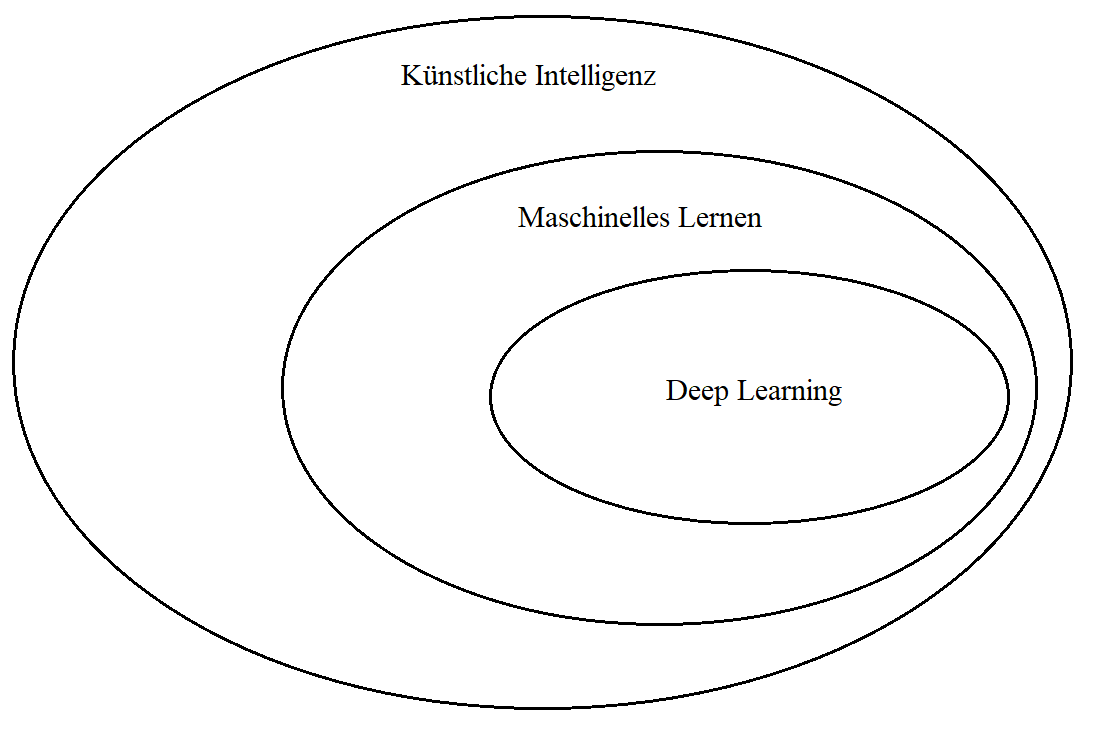
\includegraphics[width=0.9\textwidth]{images/figure_ai_venn-diagram.png}
	\caption{Ein einfaches Venn-Diagramm, das die Beziehung zwischen\\KI, ML und DL veranschaulicht.}
	\label{fig:ai-venn}
\end{figure}

Heutzutage bilden Deep Learning-Modelle die Grundlage für viele Anwendungen der Künstlichen Intelligenz, darunter Bild- und Spracherkennung, maschinelle Übersetzung, medizinische Diagnose und autonomes Fahren. Die rasante Entwicklung in diesem Bereich ist vor allem auf die Verfügbarkeit großer Datenmengen und immer leistungsfähigere Hardware zurückzuführen \parencite{Goodfellow2016deeplearning}.

\subsection{Neuronale Netze} \label{subsec:neural-networks}

% Einleitung und grundlegender Aufbau
Während die rasante Entwicklung von Deep Learning in den vergangenen Jahren besonders spürbar geworden ist, sind die zugrundeliegenden Algorithmen und Konzepte schon seit Jahrzehnten bekannt \parencite{Goodfellow2016deeplearning}. Künstliche Neuronale Netze (KNN) bilden dabei die Grundlage der allermeisten Deep Learning-Modelle. Sie sind inspiriert von der Struktur und Funktionsweise des menschlichen Gehirns und bestehen aus einer Vielzahl von miteinander verbundenen Neuronen, die in Schichten organisiert sind. Die Schichten teilen sich auf in eine Eingabeschicht (Input Layer), eine oder mehrere versteckte Schichten (Hidden Layers) und eine Ausgabeschicht (Output Layer).

%\begin{figure}[h]
%	\centering
%	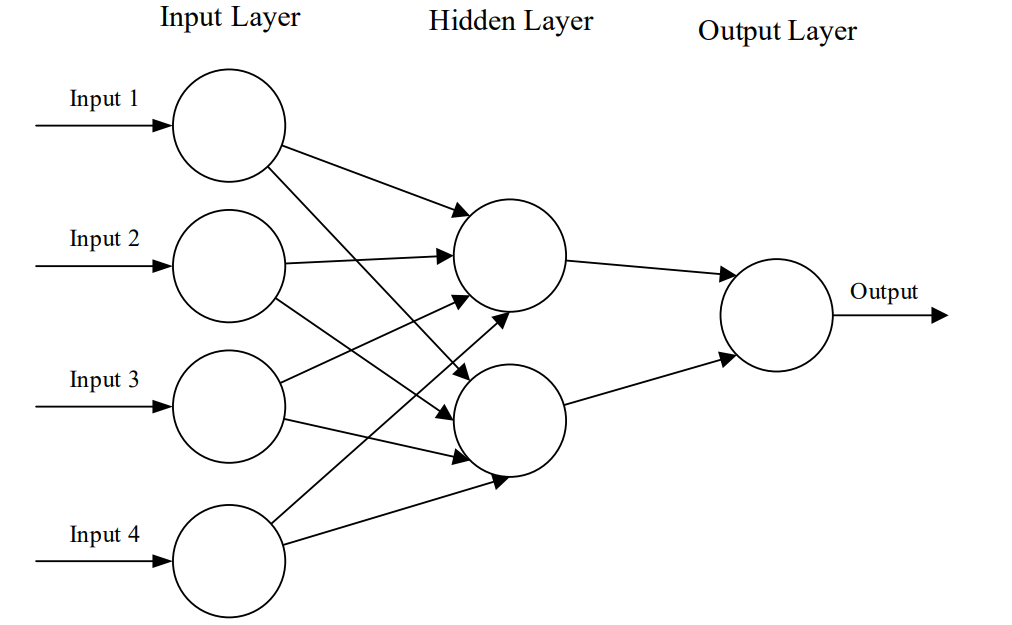
\includegraphics[width=12cm]{images/figure_ffn.png}
%	\caption{Darstellung eines einfachen neuronalen Netzes \parencite{Oshea2015cnnintro}.}
%	\label{fig:ffn}
%\end{figure}

% Einzelnes Neuron im Detail
Bei den einzelnen Neuronen handelt es sich um mathematische Modellierungen des biologischen Neurons, die erstmals in \parencite{McCulloch1943nn} vorgestellt wurden, wobei sich die heute verwendeten Neuronenmodelle kaum unterscheiden. In \autoref{fig:neuron} ist ein solches Neuronenmodell dargestellt.

\begin{figure}[h]
	\centering
	\vspace*{4mm}
	%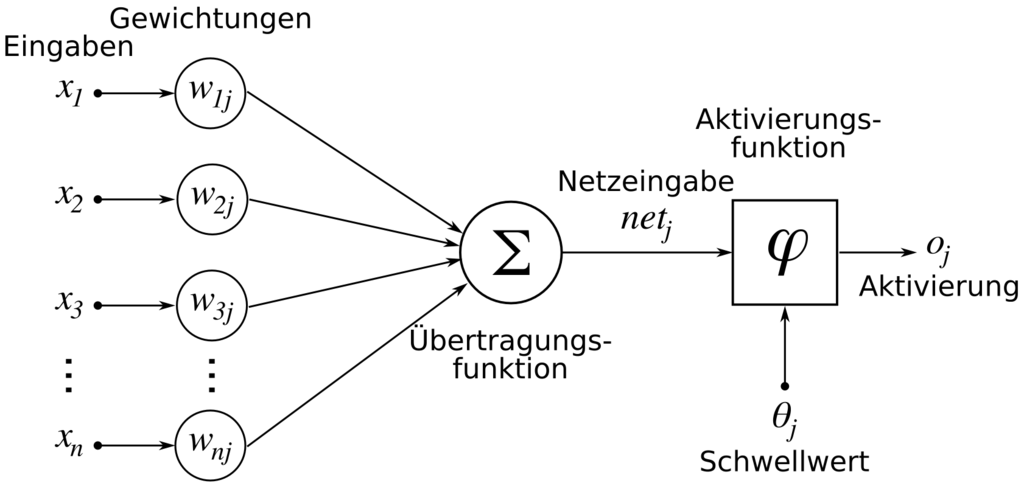
\includegraphics[width=12cm]{images/figure_mp-neuron.png}
		% Mit Beschriftung
		% https://commons.wikimedia.org/w/index.php?curid=224561
	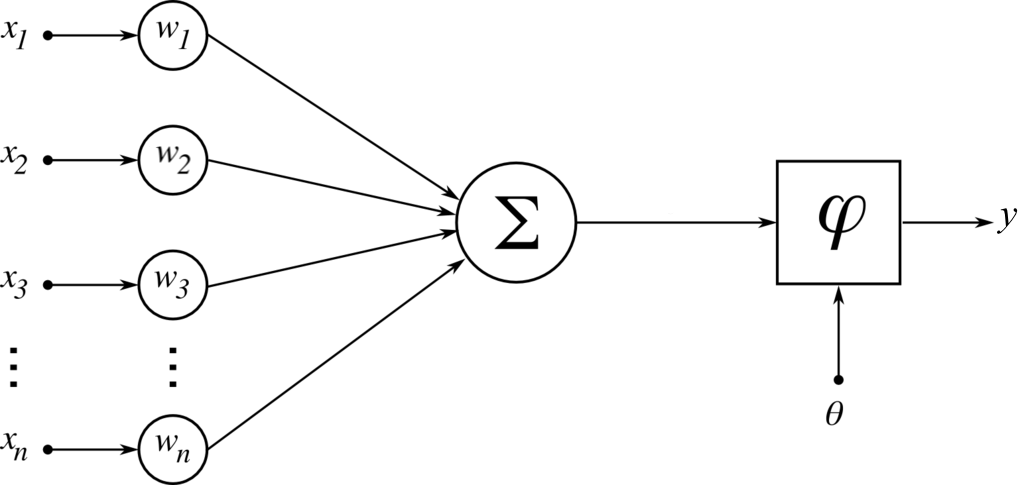
\includegraphics[width=12cm]{images/figure_mp-neuron_nd_edited1.png}
		% Ohne Beschriftung, editiert
		% https://commons.wikimedia.org/wiki/File:ArtificialNeuronModel.png
	\vspace*{2mm}
	\caption[Schematische Abbildung eines künstlichen Neurons.]{Schematische Abbildung eines künstlichen Neurons \parencite{WikiNeuronModel}.}
	\label{fig:neuron}
\end{figure}

Jedes Neuron empfängt eine Reihe von Eingaben $x_1, x_2, \dots, x_n$, entweder von externen Quellen oder von den Ausgaben anderer Neuronen. Für jede dieser Eingaben gibt es zugehörige Gewichtungen (Weights) $w_1, w_2, \dots, w_n$, welche die Stärke und Richtung (positiv oder negativ) des Einflusses der jeweiligen Eingaben auf das Neuron bestimmen. Das Neuron berechnet dann die gewichtete Summe aller Eingaben. Zusätzlich wird ein Schwellenwert (Bias) $\theta$ hinzugefügt. Die Aktivierung $y$ des Neurons kann dementsprechend wie in \autoref{eq:mp-neuron} beschrieben werden.

\begin{equation}
	y = \varphi \left( \sum_{i=1}^{n} w_{i} x_i + \theta \right),
	\label{eq:mp-neuron}
\end{equation}

wobei $\varphi$ eine Aktivierungsfunktion ist, die die Ausgabe des Neurons bestimmt. Häufig wird die Sigmoid-Funktion verwendet (siehe \autoref{eq:sigmoid}), die, im Gegensatz zu einer einfachen Schwellenwertfunktion, kontinuierlich und differenzierbar ist. Dies vereinfacht die Optimierung des Netzwerks \parencite{Zhou2021machinelearning}.

\begin{equation}
	\text{Sigmoid}(x) = \frac{1}{1 + e^{-x}}
	\label{eq:sigmoid}
\end{equation}

Die Sigmoid-Funktion eignet sich gut für binäre Klassifikationsprobleme. Für Multiklassenprobleme wird jedoch die Softmax-Funktion verwendet, die eine Wahrscheinlichkeitsverteilung über alle Klassen berechnet (siehe \autoref{eq:softmax}) \parencite{Goodfellow2016deeplearning}.

\begin{equation}
	\text{Softmax}(x)_i = \frac{e^{x_i}}{\sum_{j=1}^{N} e^{x_j}},
	\label{eq:softmax}
\end{equation}

wobei $N$ die Anzahl der Klassen ist.

% Wie neuronale Netze lernen
Im Training fließen die Eingabedaten in einer Vorwärtsausbreitung (Forward Propagation) durch das Netzwerk, um die Ausgabe zu berechnen, welche sich aus der Aktivierung der Neuronen in der Ausgabeschicht ergibt. Es wird dann eine geeignete Verlustfunktion angewendet, um den Fehler (Loss) des Modells zu berechnen. Das Ziel des Trainings ist es, die Gewichtungen der Neuronen so anzupassen, dass der Fehler minimiert wird.

% Cross Entropy
Die Wahl der Verlustfunktion hängt von der Art des Problems ab, das gelöst werden soll. Für Klassifikationsprobleme wird häufig die Kreuzentropie (Cross Entropy) verwendet, die den Fehler zwischen den tatsächlichen und den vorhergesagten Wahrscheinlichkeiten berechnet (siehe \autoref{eq:cross-entropy}).

\begin{equation}
	Loss = - \sum_{i=1}^{N} y_i \log \hat{y}_i,
	\label{eq:cross-entropy}
\end{equation}

wobei $N$ die Anzahl der Klassen ist, $y_i$ die tatsächliche Wahrscheinlichkeit für Klasse $i$ und $\hat{y}_i$ die vorhergesagte Wahrscheinlichkeit.

% Backpropagation und SGD
Die Optimierung geschieht durch eine Rückwärtsausbreitung (Backpropagation), welche den berechneten Fehler rückwärts durch das Netz propagiert, um die Gewichte und Schwellenwerte um einen geringen Wert in die Richtung anzupassen, die den Fehler minimieren würde. Die Richtung wird bestimmt, indem der Gradient der Verlustfunktion berechnet wird. Die Lernrate (Learning Rate) bestimmt, wie groß die Schritte sind, die entlang des Gradienten gemacht werden. So bewegt sich das Modell iterativ entlang des Gradienten hin zu einem lokalen Minimum der Verlustfunktion. Dieser Algorithmus wird als Gradient Descent (Gradientenabstieg) bezeichnet. Im Maschinellen Lernen kommt hauptsächlich der Stochastic Gradient Descent (SGD) zum Einsatz, der immer nur einen kleinen, zufällig ausgewählten Teil der Trainingsdaten (einen sogenannten Batch) verwendet, um den Gradienten zu berechnen.

% CNN als Beispiel eines Deep Learning-Modells
\begin{figure}[t]
	\centering
	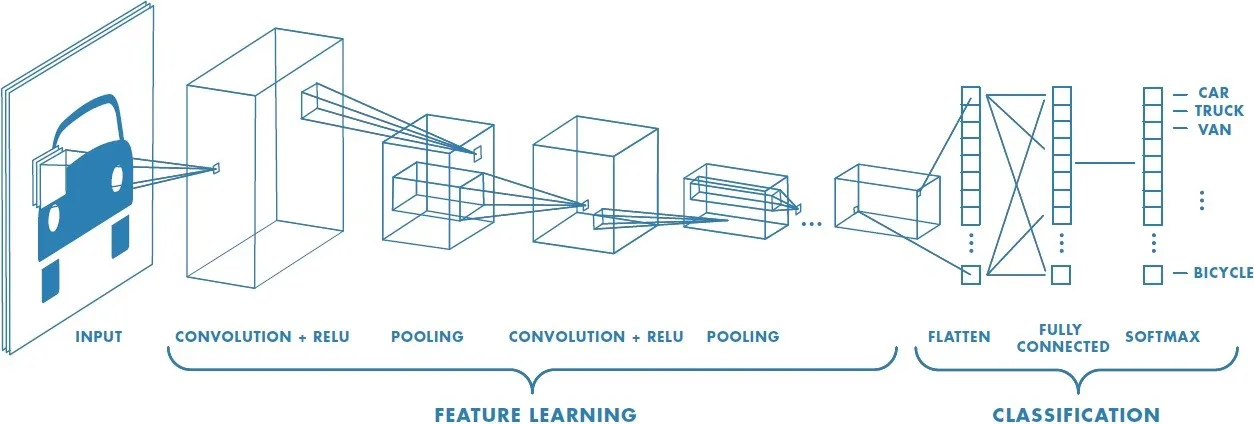
\includegraphics[width=\textwidth]{images/figure_cnn.png}
	\caption[Architektur eines Convolutional Neural Networks.]{Architektur eines Convolutional Neural Networks \parencite{Saha2018cnnfigure}.}
	\label{fig:cnn}
\end{figure}

% CNN als Deep Learning-Beispiel eines NN
Deep Learning mit neuronalen Netzen kann gut am Beispiel des Convolutional Neural Networks (CNN) veranschaulicht werden, welches speziell für die Verarbeitung von Bildern entwickelt wurde (siehe \autoref{fig:cnn}). Mit Backpropagation trainierte CNNs wurden erstmals in \parencite{LeCun1989cnnbackprop} behandelt, bilden aber auch heute noch die Grundlage von zahlreichen Anwendungen im ML.

Ein CNN besteht aus mehreren Schichten, darunter Convolutional Layers, Pooling Layers und Fully Connected Layers. Die Convolutional Layers extrahieren sogenannte \emph{Feature Maps} aus den Eingabebildern, indem sie Faltungskerne über das Bild schieben und die gewichteten Summen der Pixel berechnen. Die Pooling Layers reduzieren die Dimensionalität der Feature Maps und die Fully Connected Layers kombinieren die extrahierten Features, um die endgültige Klassifikation vorzunehmen. Dadurch berücksichtigen sie auf effektive Weise die räumliche Struktur von Bildern und können benötigen dabei weniger Parameter als herkömmliche neuronale Netze \parencite{Goodfellow2016deeplearning}.

\subsection{Datenaugmentation} \label{subsec:data-augmentation}

% Overfitting
Wenn ein Modell so stark an die Trainingsdaten angepasst wird, dass es nicht in der Lage ist, auf neuen, unbekannten Daten zu generalisieren, spricht man von Overfitting \parencite{Goodfellow2016deeplearning}. Statt die zugrundeliegenden Muster zu lernen, speichert das Modell auch zufällige Rauschsignale und Fehler. Dies führt dazu, dass das Modell auf den Trainingsdaten eine hohe Genauigkeit erreicht, aber auf neuen Daten eine schlechtere Leistung zeigt. Man verwendet daher neben den Trainingsdaten auch Validierungsdaten (Daten, die nicht zum Training des Modells verwendet werden) zur Überwachung des Overfittings.

% Overfitting kann das Resultat einer zu hohen Komplexität des Modells sein, die dafür sorgt, dass die Trainingsdaten zu genau modelliert werden. Techniken zur Regularisierung zielen deshalb darauf ab, die optimale Komplexität eines Modells zu finden. Dropout \parencite{Srivastava2014dropout} ist eine solche Technik, bei der zufällig ausgewählte Neuronen während des Trainings deaktiviert werden, um zu verhindern, dass das Modell sich auf spezifische Merkmale verlässt. Als Early Stopping wird ein anderer Ansatz bezeichnet, bei dem das Training beendet wird, wenn die Leistung auf den Validierungsdaten beginnt, sich zu verschlechtern.
Während Overfitting auch das Resultat einer zu hohen Komplexität des Modells sein kann, die dafür sorgt, dass die Trainingsdaten zu genau modelliert werden, liegt das Problem oftmals in der Quantität und Qualität der Trainingsdaten selbst. Sind nicht genügend Daten vorhanden, oder sind die Daten nicht divers genug, kann das Modell nicht generalisieren.

% Datenaugmentation
Dabei kann das Modell auch ohne völlig neue Daten zu beschaffen robuster gegenüber Variationen gemacht werden, indem es mit leicht veränderten Versionen der Trainingsdaten trainiert wird. Bei der Datenaugmentation werden unterschiedliche Transformationen auf die vorhandenen Daten angewendet, z.B. Rotation, Skalierung, Verschiebung, Spiegelung, Helligkeitsanpassung oder Rauschen \parencite{Shorten2019dataaugmentation}. Die Transofrmationen werden meist zufällig parametrisiert, um eine Vielzahl von Variationen zu erzeugen. Das Ziel ist es, das Modell zu zwingen, die zugrundeliegenden Muster der Daten zu lernen, anstatt sich auf spezifische Merkmale zu verlassen, die nur in den Trainingsdaten vorhanden sind. Einige Beispiele für Datenaugmentationstechniken sind in \autoref{fig:data-augmentation} dargestellt.

Datenaugmentation hat sich als eine der wichtigsten Ansätze zur Vermeidung von Overfitting und zur Verbesserung der Generalisierungsfähigkeit von Modellen erwiesen. Sie findet in fast allen Methoden des Maschinellen Lernens Anwendung.

% Beispiele
\begin{figure}[t]
	\centering
	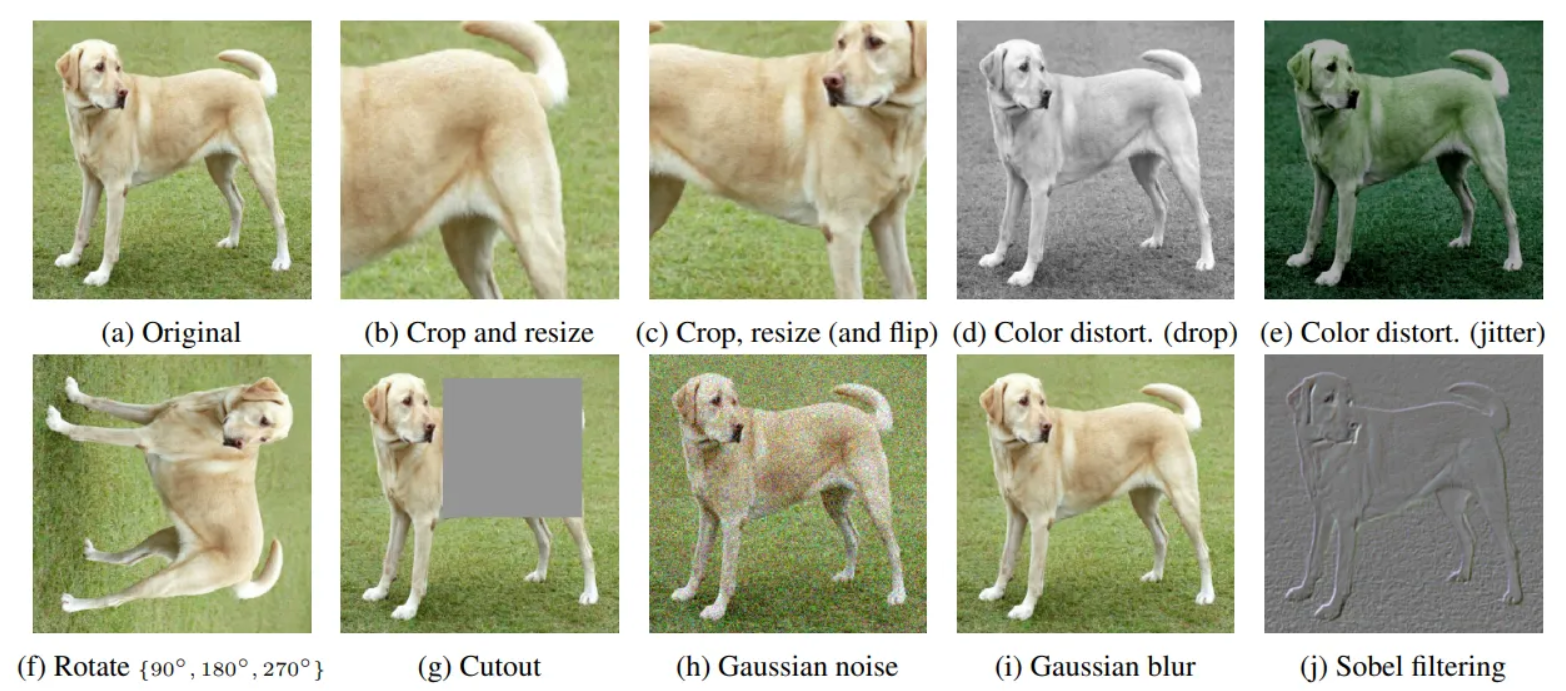
\includegraphics[width=\textwidth]{images/figure_data_augmentation.png}
	\caption{Einige Beispiele für unterschiedliche Datenaugmentationstechniken\\
	und Kombinationen, die in \parencite{Chen2020simclr} verwendet wurden.}
	\label{fig:data-augmentation}
\end{figure}

\subsection{Out-of-Distribution Daten} \label{subsec:ood}

% Definition und Problematik
Wenn ein KI-Modell mit Daten konfrontiert wird, die außerhalb des Bereichs liegen, den es während des Trainings gesehen hat, spricht man von Out-of-Distribution (OOD)-Daten. Es handelt sich also um Datenpunkte oder Muster, die sich signifikant von den Trainingsdaten unterscheiden. Dies kann zu Problemen führen, da das Modell möglicherweise nicht in der Lage ist, angemessene Vorhersagen oder Entscheidungen für diese Daten zu treffen. Die Erkennung von OOD-Daten ist daher ein wichtiges Forschungsgebiet im maschinellen Lernen, da sie dazu beitragen kann, die Zuverlässigkeit und Sicherheit von KI-Systemen zu verbessern.

% Schwellenwert
Grundsätzlich sollte ein Neuronales Netz höhere Softmax-Wahrscheinlichkeiten für In-Distribution (ID)-Daten und niedrigere Wahrscheinlichkeiten für OOD-Daten ausgeben. Tatsächlich sind die Wahrscheinlichkeiten für OOD-Daten fast immer sehr hoch, meist reicht aber der Abstand zwischen ID- und OOD-Daten aus, um OOD-Instanzen frühzeitig zu identifizieren \parencite{Hendrycks2018baselineooddetection}.

% Andere Ansätze
Oftmals ist die OOD-Detektion aber weniger trivial, etwa wenn sich ID- und OOD-Daten sehr ähnlich sind. Es wird daher stets nach alternativen Ansätzen gesucht, um die OOD-Detektion zu verbessern. In \parencite{Hendrycks2018baselineooddetection} wird beispielsweise ein Klassifikator erweitert, um Rekonstruktionen der Eingabedaten zu erstellen und den Fehler zwischen den Original- und Rekonstruktionsdaten zu messen. Ein hoher Rekonstruktionsfehler kann auf OOD-Daten hinweisen. %Auch das Temperature Scaling \parencite{Guo2017tempscaling}, welches die Softmax-Wahrscheinlichkeiten kalibriert und somit den Abstand zwischen ID- und OOD-Daten vergrößert, kann zusammen mit kleinen Störungen in den Eingabedaten für zuverlässigere OOD-Detektion sorgen \parencite{Liang2020odin}.

\section{Synthetische Daten} \label{sec:synt-data}

% Anschließend an Datenaugmentation; Problematik der Datensammlung
Datenaugmentation wurde bereits als eine Möglichkeit vorgestellt, um die Menge und Vielfalt der Trainingsdaten zu erhöhen und damit die Generalisierungsfähigkeit des Modells zu verbessern. Allerdings kann die bloße Augmentation an ihre Grenzen stoßen, wenn die verfügbaren Trainingsdaten selbst nicht genügend Vielfalt aufweisen. In solchen Fällen können synthetische Daten eine nützliche Ergänzung sein. Anstatt einfache Transformationen auf die Eingangsdaten anzuwenden, werden völlig neue Datenpunkte generiert, die die zugrundeliegenden Muster der realen Daten nachahmen. Auch im Hinblick auf den Datenschutz sind synthetische Daten vielversprechend, da sie die Möglichkeit bieten, sensible und personenbezogene Informationen zu schützen.

% Fortschritte in generativer Modellierung durch Deep Learning
Während synthetische Daten auch manuell mit Hilfe von Simulationssoftware erstellt werden können, hat insbesondere die Entwicklung generativer KI-Modelle in den letzten Jahren zu einer neuen Ära der synthetischen Datenerzeugung geführt. Diese Modelle sind in der Lage, komplexe Datenstrukturen zu lernen und realistische Daten zu generieren, die von echten Daten kaum zu unterscheiden sind.
% Diese Entwicklung der generativen Modellierung ergibt sich vor allem aus den Fortschritten im Deep Learning \parencite{Foster2020gendeeplearning}: Als Hierarchie der Mustererkennung können Deep Learning-Modelle das hohe Maß bedingter Abhängigkeiten zwischen Merkmalen in den Daten lernen und reproduzieren. Und als Form des Representation Learning erleichtert Deep Learning die Generierung von Daten, indem nur eine geeignete niedrigdimensionale Repräsentation gewählt werden muss, welches das Modell wieder zu einer realistischen Dateninstanz umwandeln soll.

% Einleitung folgender Abschnitte
Da sich diese Arbeit mit der Bildklassifikation beschäftigt, wird im Folgenden vor allem auf generative Modelle eingegangen, die darauf spezialisiert sind, Bilder zu generieren. Es sollen einige der wichtigsten Modelle vorgestellt werden, um eine Grundlage für den aktuellen Stand der synthetischen Datengenerierung zu schaffen.

\subsection{Variational Autoencoder} \label{subsec:vae}

Ein Autoencoder ist eine spezielle Art von KI-Modell, das entwickelt wurde, um Daten effizient zu komprimieren und anschließend zu rekonstruieren. Es wurde im Wesentlichen in \parencite{Hinton2006autoencoder} vorgestellt, die Grundideen gehen jedoch bis in die 1980er Jahre zurück, wie z.B. in \parencite{Rumelhart1986backpropagation}, wo auch das Backpropagation-Verfahren zur Optimierung neuronaler Netze beschrieben wurde.

Autoencoder bestehen aus zwei Hauptkomponenten; einem \emph{Encoder}, der die Eingabedaten in einen niedrigdimensionalen Darstellungsvektor komprimiert, und einem \emph{Decoder}, der den Darstellungsvektor wieder in die ursprünglichen Daten umwandelt. So wird das Originalbild als Punkt in einem mehrdimensionalen latenten Raum abgebildet, in dem jede Dimension eine bestimmte Eigenschaft des Bildes kodiert.

\begin{figure}[h]
	\centering
	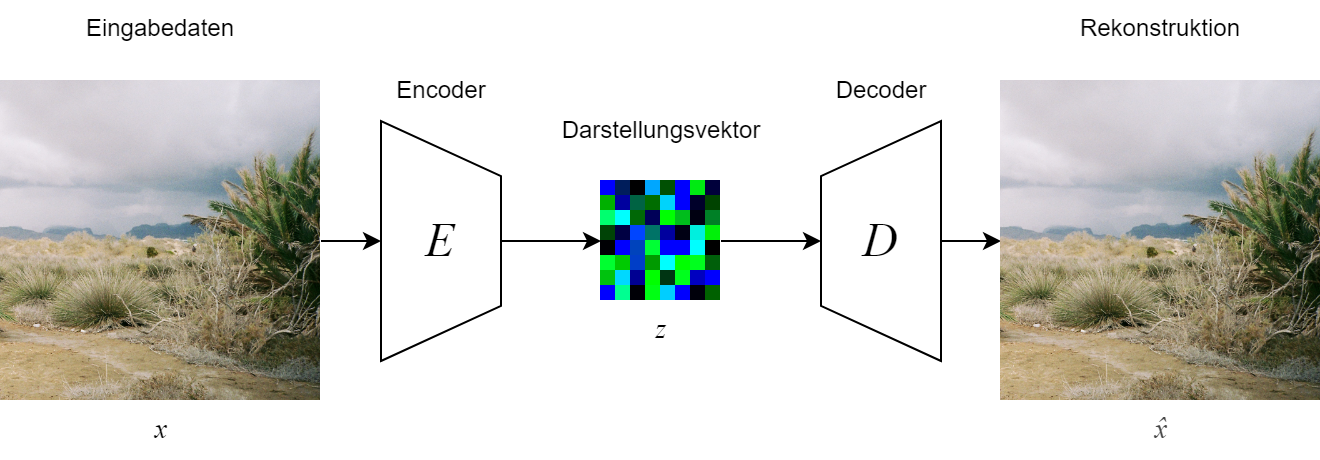
\includegraphics[width=0.8\textwidth]{images/figure_autoencoder.png}
	\caption{Aufbau eines Autoencoders.}
	\label{fig:autoencoder}
\end{figure}

Das Training eines Autoencoders erfolgt durch Minimierung des Rekonstruktionsfehlers, der die Differenz zwischen den Eingabedaten und den Rekonstruktionen beschreibt. Eine gängige Verlustfunktion hierfür ist der Mean Squared Error (MSE), der in \autoref{eq:loss-mse} formuliert ist.

\begin{equation}
	Loss=\frac{1}{n}\sum_{i=1}^n (x_i-\hat{x}_i)^2,
	\label{eq:loss-mse}
\end{equation}

wobei $x_i$ die Eingabedaten und $\hat{x}_i$ die Rekonstruktionen sind.

% Weiterentwicklung durch VAE
Autoencoder können theoretisch zur Generierung synthetischer Daten verwendet werden, indem ein beliebiger Punkt im latenten Raum gewählt und durch den Decoder rekonstruiert wird. Allerdings hat der herkömmliche Autoencoder einige Schwächen in Bezug auf diese Aufgabe \parencite{Foster2020gendeeplearning}: Da er immer nur einen festen Punkt im latenten Raum für jede Eingabe lernt, entsteht ein diskreter und unstrukturierter latenter Raum. Es ist weder die Kontinuierlichkeit zwischen den Punkten der Eingabedaten noch die Vollständigkeit des latenten Raums sichergestellt, sodass neue Stichproben aus dem latenten Raum nicht unbedingt realistische Daten erzeugen.

Der \emph{Variational Autoencoder} (VAE) \parencite{Kingma2013vae} adressiert die Schwachstellen des Autoencoders und verwendet probabilistische Methoden, um die Datenverteilung im latenten Raum zu modellieren; anstelle eines einzelnen, festen Punktes im latenten Raum wird für jede Eingabe eine Verteilung gelernt, aus der die latenten Variablen stammen. Die Verteilung entspricht dabei einer einfachen, bekannten Verteilung, wie z.B. einer Normalverteilung $\mathcal{N}(0,1)$.

Um die Verteilungen zu lernen, berechnet der Encoder einerseits den Mittelwert $\mu$ und die Standardabweichung $\sigma$, und erzeugt außerdem eine zufällige Stichprobe der Verteilung. Der Decoder nimmt diese Stichprobe und rekonstruiert die Eingabedaten. Beim Training wird nicht nur der Rekonstruktionsfehler minimiert, sondern auch die sogenannte Kullback-Leibler-Divergenz (KL-Divergenz), welche die Ähnlichkeit zwischen zwei Wahrscheinlichkeitsverteilungen $Q$ und $P$ misst (siehe \autoref{eq:kl-divergence}), in diesem Fall zwischen der latenten Verteilung und einer Normalverteilung (siehe \autoref{eq:kl-divergence-vae}) \parencite{Foster2020gendeeplearning}.

\begin{equation}
	D_{KL}\left(Q || P\right) = \int q(x) \log \frac{q(x)}{p(x)}dx
	\label{eq:kl-divergence}
\end{equation}
\begin{equation}
	D_{KL}\left(\mathcal{N}(\mu,\sigma) || \mathcal{N}(0,1)\right) = \frac{1}{2} \sum (1 + \log(\sigma^2) - \mu^2 - \sigma^2)
	\label{eq:kl-divergence-vae}
\end{equation}

Durch die Kombination von Rekonstruktionsfehler und KL-Divergenz ergibt sich nun eine Annäherung an die die Log-Likelihood $\log p(x)$ der Daten, also der Wahrscheinlichkeit, dass das Modell die Eingabedaten korrekt rekonstruiert. Diese Annäherung wird als Evidence Lower Bound (ELBO) bezeichnet. Sie ist deshalb notwendig, weil zur direkten Berechnung der Log-Likelihood die Integration über alle möglichen Werte der latenten Variablen $z$ erforderlich wäre, was in der Praxis nicht möglich ist.

Die finale Verlustfunktion, die sowohl den Rekonstruktionsfehler als auch die KL-Divergenz kombiniert, ergibt sich aus der negativen ELBO (siehe \autoref{eq:vae-loss}). Diese Verlustfunktion wird minimiert, um sowohl die Qualität der Rekonstruktionen zu maximieren als auch die latente Verteilung näher an die Normalverteilung anzunähern.

\begin{equation}
	Loss = -\mathbb{E}{q(z|x)}[\log p(x|z)] + D_{KL}(q(z|x) || p(z)),
	\label{eq:vae-loss}
\end{equation}

wobei $p(z|x)$ die latente Verteilung eines gegebenen Datenpunktes $x$, $p(x|z)$ die Rekonstruktion des Datenpunktes $x$ aus der latenten Darstellung $z$ und $p(z)$ die Prior-Verteilung der latenten Variablen ist.

% Trotz ihres Erfolgs haben auch VAEs einige Nachteile, da ihre zugrundeliegende Architektur ein sogenanntes Bottleneck-Problem aufweist, bei dem alle Informationen in den latenten Variablen komprimiert werden müssen. Es gehen zwangsweise Informationen verloren, was zu einer ungenauen Rekonstruktion der Eingabedaten führen kann. Darüber hinaus kann die Modellierung der Datenverteilung im latenten Raum schwierig sein, insbesondere bei komplexen Datenstrukturen. \parencite{Zhou2021machinelearning} %?

\subsection{Generative Adversarial Networks} \label{subsec:gan}

Ein weiteres berühmtes KI-Modell ist das \emph{Generative Adversarial Network} (GAN), das in \parencite{Goodfellow2014gan} vorgestellt wurde. GANs bestehen aus einem \emph{Generator}- und einem \emph{Diskriminator}-Modell, die in einem adversariellen Prozess gegeneinander antreten.

Der Generator nimmt Zufallsrauschen als Eingabe und erzeugt daraus Daten, die möglichst realistisch wirken sollen. Der Diskriminator erhält sowohl echte Daten aus dem Trainingsdatensatz als auch die vom Generator erzeugten Daten. Seine Aufgabe ist es, zwischen echten und künstlichen Daten zu unterscheiden. Dafür gibt er für einen gegebenen Datenpunkt die Wahrscheinlichkeit aus, dass dieser echt ist. \autoref{fig:gan} gibt einen Überblick über das ganze System.

\begin{figure}[h]
	\centering
	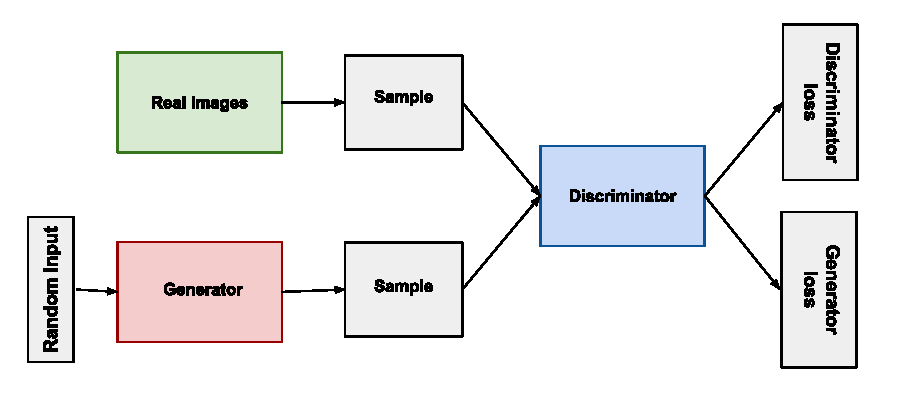
\includegraphics[width=\textwidth]{images/figure_gan.pdf}
	\caption[Überblick über das GAN-Training.]{Überblick über das GAN-Training \parencite{GoogleDev2022ganfigure}.}
	\label{fig:gan}
\end{figure}

Der Diskriminatorverlust ergibt sich aus der Differenz zwischen der Wahrscheinlichkeit, dass echte Daten als echt und künstliche Daten als falsch klassifiziert werden. Der Generatorverlust ergibt sich aus der Differenz zwischen der Wahrscheinlichkeit, dass künstliche Daten als echt klassifiziert werden und der tatsächlichen Wahrscheinlichkeit, dass sie echt sind. Die Verlustfunktionen für den Generator und den Diskriminator sind in \autoref{eq:gan-loss} formuliert.

\begin{equation}
	\begin{aligned}
		Loss_D &= -\mathbb{E}_{x \sim P}[\log D(x)] - \mathbb{E}_{z \sim P(z)}[\log(1 - D(G(z)))] \\
		Loss_G &= -\mathbb{E}_{z \sim P(z)}[\log D(G(z))]
	\end{aligned}
	\label{eq:gan-loss}
\end{equation}

% Vorteile & Nachteile
Besonders in der Bildgenerierung haben GANs eine hohe Qualität erreicht. GANs sind auch flexibel in Bezug auf die Eingangsdaten und können mit verschiedenen Datentypen wie Bildern, Texten oder Audiodaten arbeiten. Dennoch gibt es einige Nachteile. Beispielsweise kann das Training eines GANs sehr instabil sein, da es schwierig ist, ein Gleichgewicht zwischen Generator und Diskriminator zu finden. Es kann auch zum sogenannten Modus-Kollaps kommen, bei dem der Generator nur eine begrenzte Anzahl von Beispielen erzeugt, da der Diskriminator diese als besonders realistisch bewertet \parencite{Foster2020gendeeplearning}. Der Generator lernt dann, nur diese Beispiele zu reproduzieren, anstatt die gesamte Datenverteilung zu lernen. Auch die Wahl geeigneter Hyperparameter ist eine Herausforderung.

\subsection{Diffusionsmodelle} \label{subsec:diffusion-models}

% Einleitung, Konzept der Diffusion
In den letzten Jahren haben Diffusionsmodelle zu einem enormen Fortschritt in der Bildgenerierung, insbesondere der Text-to-Image (T2I)-Generierung, geführt. Diese Modelle basieren auf dem Konzept der Diffusion, das den Prozess der langsamen Vermischung von Teilchen oder Informationen über die Zeit beschreibt. Im maschinellen Lernen fand das Konzept erstmals in \parencite{SohlDickstein2015diffusionmodels} Anwendung, mit der Idee, die Struktur von Daten durch Hinzufügen von Rauschen schrittweise aufzulösen und anschließend ein Modell darauf zu trainieren, das ursprüngliche Bild zu rekonstruieren (siehe \autoref{fig:regular-diffusion}). Seitdem haben sich Diffusionsmodelle als eine neue Klasse von generativen Deep Learning-Modellen etabliert, die in der Lage sind, noch realistischere Bilder zu generieren als GANs.

% Vorwärts- und Rückwärtsdiffusion
\begin{figure}[h]
	\centering
	\includegraphics[width=12cm]{images/figure_diffusion_image_custom.png}
	\caption[Darstellung der Vorwärts- und Rückwärtsdiffusion in einem Diffusionsmodell.]{Darstellung der Vorwärts- und Rückwärtsdiffusion in einem Diffusionsmodell.}
	\label{fig:regular-diffusion}
\end{figure}

Das Training von Diffusionsmodelle teilt sich in zwei Phasen auf, die Vorwärts- und die Rückwärtsdiffusion, welche beide als Markov-Ketten modelliert werden können, also stochastische Prozesse, bei denen die zukünftige Entwicklung eines Systems nur von seinem aktuellen Zustand abhängt. Im Bezug auf Diffusionsmodelle repräsentiert jeder Schritt in der Markov-Kette einen Zeitschritt $t$ und die Zustände $x^{(t)}$ sind die Bilder zu diesem Zeitschritt.

In der Vorwärtsdiffusion fügt das Modell einem Bild schrittweise Rauschen hinzu, sodass es sich am Ende des Prozesses wie eine Normalverteilung verhält. Die Wahrscheinlichkeitsdichte des verrauschten Bildes wird durch die Produktregel der bedingten Wahrscheinlichkeiten berechnet (siehe \autoref{eq:forward-diffusion}).

\begin{equation}
	q \left( x^{(0 \dots T)} \right) = q \left(x^{(0)}\right)\prod_{t=1}^T q \left(x^{(t)}|x^{(t-1)}\right)
	\label{eq:forward-diffusion}
\end{equation}

In der Rückwärtsdiffusion wird das Modell darauf trainiert, das verrauschte Bild schrittweise in das ursprüngliche Bild zurückzuwandeln. Die Wahrscheinlichkeitsdichte des ursprünglichen Bildes wird ebenfalls durch die Produktregel der bedingten Wahrscheinlichkeiten berechnet (siehe \autoref{eq:reverse-diffusion}).

\begin{equation}
	p \left( x^{(0 \dots T)} \right) = p \left(x^{(T)}\right)\prod_{t=1}^T p \left(x^{(t-1)}|x^{(t)}\right)
	\label{eq:reverse-diffusion}
\end{equation}

Das Neuronale Netz, das zur Vorhersage der Zustände $x^{(t-1)}$ aus den verrauschten Zuständen $x^{(t)}$ verwendet wird, ist typischerweise ein Denoising U-Net (siehe \autoref{fig:regular-diffusion}). Es hat eine ähnliche Struktur wie ein Autoencoder, wobei Skip Connections zwischen den Encoder- und Decoder-Schichten bestehen, um die Rekonstruktion des ursprünglichen Bildes zu verbessern. Die Hauptaufgabe des U-Nets besteht darin, das hinzugefügte Rauschen zu schätzen, welches anschließend subtrahiert wird, um das ursprüngliche Bild zu rekonstruieren.

Die Verlustfunktion wird oft als MSE formuliert, um den Unterschied zwischen dem generierten Rauschen und dem tatsächlichen Rauschen zu minimieren.

Anders als bei GANs gibt es keine direkten adversarialen Optimierungsmechanismen, die zu einem Ungleichgewicht führen können. Es wird stattdessen explizit die Wahrscheinlichkeitsdichte zwischen den realen Daten und den erzeugten Daten minimiert, was zu einem robusteren und stabileren Trainingsprozess führt.

% DALL-E (2) für Text-to-Image
Eine entscheidende Weiterentwicklung der Diffusionsmodelle war die Text-Konditionierung des generativen Prozesses. In \parencite{Ramesh2022dalle2} wurde \emph{DALL-E 2} vorgestellt, welches ein Diffusionsmodell verwendet, das in der Lage ist, Bilder aus Textbeschreibungen zu generieren. DALL-E 2 verwendet das Transformer-Modell \parencite{Vaswani2017transformer}, um die Textbeschreibungen in eine latente Repräsentation zu kodieren, die dann im Diffusionsprozess verwendet wird.

% Stable Diffusion
\emph{Stable Diffusion} ist ein besonders einflussreiches Diffusionsmodell, das sich durch die Verwendung eines latenten Diffusionsprozesses auszeichnet \parencite{Rombach2022stablediffusion}. Anstatt den Diffusionsprozess direkt auf den hochdimensionalen Bildraum anzuwenden, führt Stable Diffusion die Diffusion in einem niedrigdimensionalen latenten Raum durch, der durch ein VAE-ähnliches Netzwerk generiert wird (siehe \autoref{fig:stable-diffusion}). Diese Technik reduziert die Rechenkosten und beschleunigt den Generierungsprozess erheblich, während gleichzeitig hochauflösende und realistische Bilder erzeugt werden.

\begin{figure}[t]
	\centering
	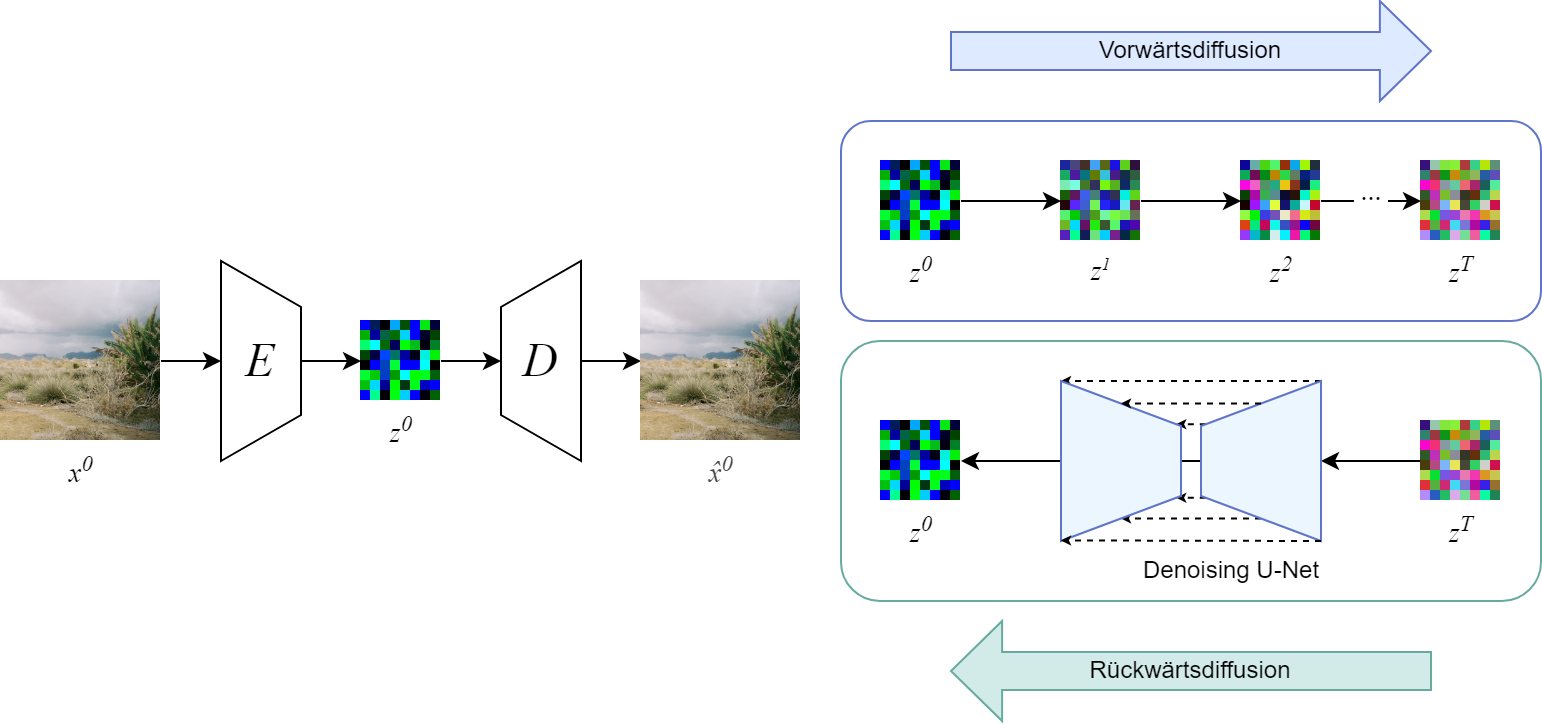
\includegraphics[width=\textwidth]{images/figure_diffusion_merged_custom.png}
	\caption[Darstellung der Vorwärts- und Rückwärtsdiffusion in Stable Diffusion.]{Darstellung der Vorwärts- und Rückwärtsdiffusion in Stable Diffusion:\\
		Die	Diffusionsprozesse werden auf die latenten Darstellungen der Bilder\\
		angewendet (rechts), welche vorher mit einem VAE encodiert wurden (links).}
	\label{fig:stable-diffusion}
\end{figure}

%\newpage

\subsection{DA-Fusion} \label{subsec:da-fusion}

% Einleitung; Kurze Beschreibung, Versprechen der Methode
\emph{DA-Fusion} \parencite{Trabucco2023dafusion} ordnet sich zwischen den Bereichen der Datenaugmentation und der synthetischen Datengenerierung ein. Es handelt sich um eine Methode zur semantischen Datenaugmentation von Bildern unter Verwendung eines vortrainierten Stable Diffusion-Modells. 

Der traditionelle Ansatz der Datenaugmentation, wie in \autoref{subsec:data-augmentation} beschrieben, hat sich als effektiv erwiesen, um die Generalisierungsfähigkeit von Modellen zu verbessern. Allerdings erfordert dieser Ansatz auch eine gute Intuition in Bezug auf den verwendeten Datensatz, um zu vermeiden, dass Transformationen gewählt werden, durch die Informationen verloren gehen, die für die Aufgabe des zu trainierenden Modells wichtig sind. Wenn beispielsweise Farbinformationen für die Klassifizierung von Blumen wichtig sind, könnte die Datenaugmentation durch zufällige Farbänderungen die Leistung des Modells verschlechtern. Ein weiteres Beispiel sind Objekte, die klein im Bild sind und durch zufällige Ausschnitte des Bildes aus der Sicht des Modells verschwinden können. DA-Fusion hingegen nutzt das Wissen eines vortrainierten Diffusionsmodelle, um den Bildinhalt semantisch zu verstehen und automatisch neue, realistische Variationen zu generieren.

%\begin{figure}[h]
%	\centering
%	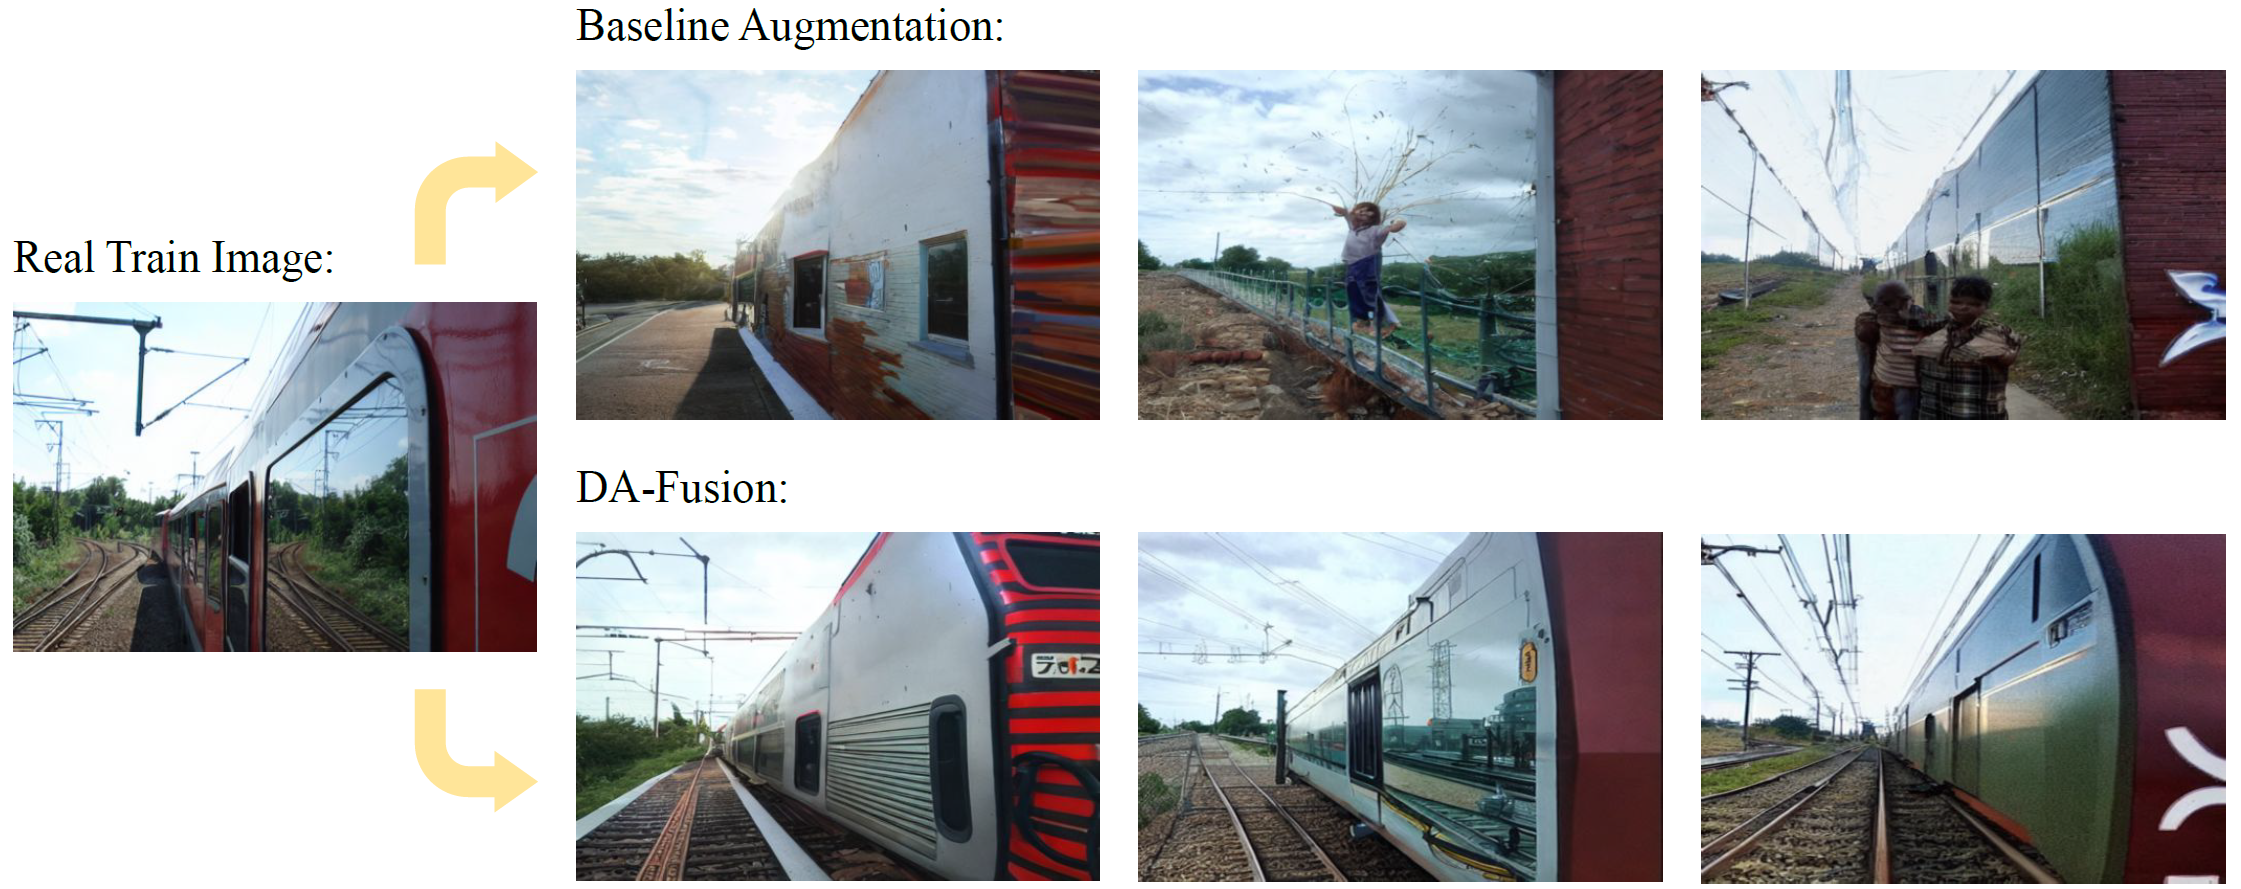
\includegraphics[width=\textwidth]{images/figure_da-fusion_vs_baseline.png}
%	\caption[Vergleich zwischen semantischen Augmentationen aus Baseline-Methode und DA-Fusion.]{Vergleich zwischen semantischen Augmentationen aus Baseline-Methode\\
%	und DA-Fusion \parencite{Trabucco2023dafusion}.}
%	\label{fig:da-fusion-baseline}
%\end{figure}

% Fine-tuning mit Textual Inversion
Dafür wird zunächst die Methode Textual Inversion aus \parencite{Gal2022textualinversion} angewendet, um ein vortrainiertes Stable Diffusion-Modell auf den gegebenen Datensatz feinabzustimmen (Fine-tuning). Für jedes Konzept bzw. für jede Klasse wird ein neues Text-Embedding \lstinline|<y>| als Platzhalter in das Modell integriert, das unter Verwendung von Trainings-Prompts wie \lstinline|"a photo of a <y>"| und den zugehörigen Bilddaten trainiert wird. Entscheidend ist hier, dass nicht das ganze Diffusionsmodell neu trainiert wird, sondern lediglich neue wörter erlernt werden, welche die spezifischen Konzepte repräsentieren, sodass sich bei der Bildgenerierung weiterhin auf das vortrainierte semantische Wissens des Modells gestützt werden kann (siehe \autoref{fig:da-fusion-process}).

\begin{figure}[t]
	\centering
	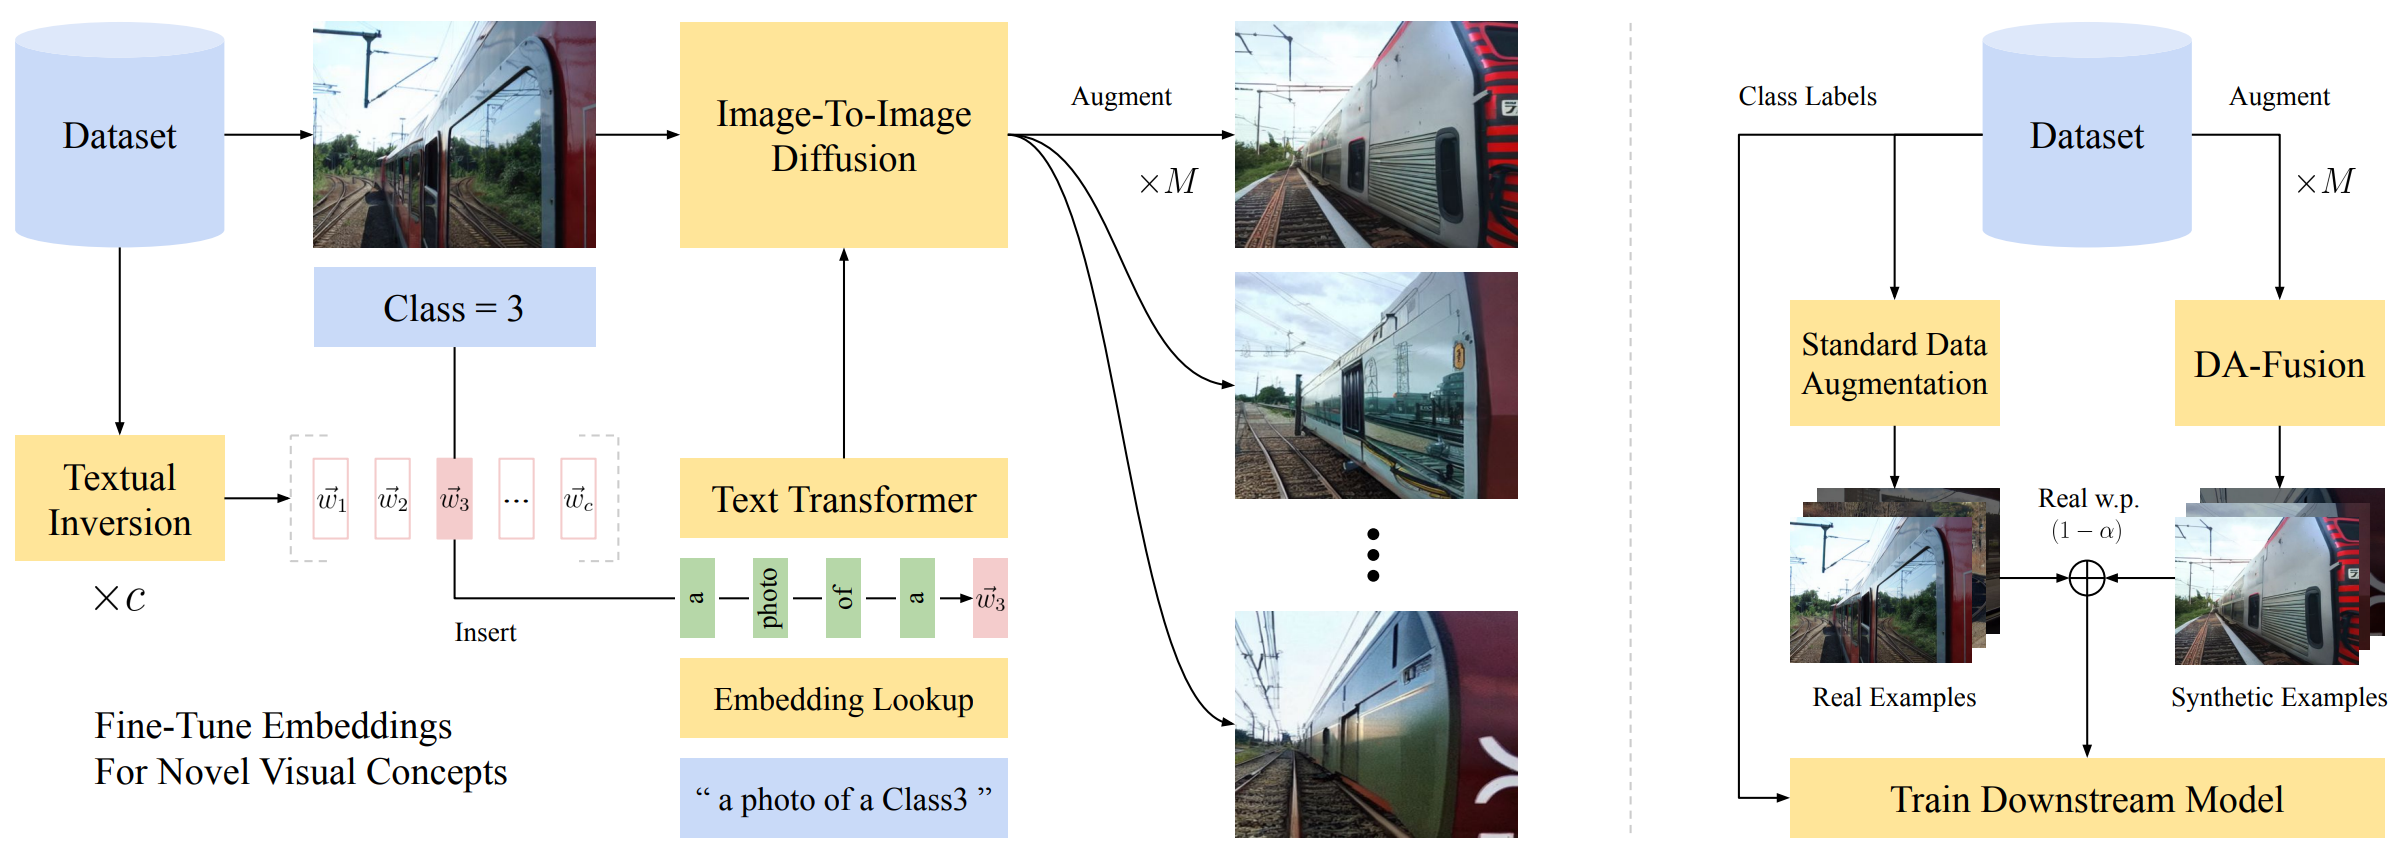
\includegraphics[width=\textwidth]{images/figure_da-fusion_architecture.png}
	\caption[Überblick über den Prozess zur Datenaugmentation mit DA-Fusion.]{Überblick über den Prozess zur Datenaugmentation mit\\
	DA-Fusion \parencite{Trabucco2023dafusion}.}
	\label{fig:da-fusion-process}
\end{figure}

% Prozess der Datengenerierung
Anschließend können die Bilder augmentiert werden, indem ihnen eine geringe Menge an Rauschen hinzugefügt wird (also ein Prozess der Vorwärtsdiffusion), welches dann durch das feinabgestimmte Modell wieder entfernt werden soll (die Rückwärtsdiffusion, die von dem Modell gelernt wurde). Hier kommen die selben Text-Prompts zum Einsatz, welche die Text-Embeddings der Konzepte beinhalten. Auf diese Weise müssen keine völlig neuen Bilder generiert werden, denn die grundlegende Struktur wird durch die ursprünglichen Bilder vorgegeben. Dieser Prozess bietet die Möglichkeit, den Grad der Augmentation durch die Wahl des Zeitschritts $t$ zu steuern, an dem das Bild in die Rückwärtsdiffusion eingefügt wird und wie stark es dafür vorher verrauscht werden muss. So entstehen stärkere oder subtilere Augmentationen.

% Basically SDEdit but with fine-tuned tokens
Der beschriebene Image-to-Image-Generierungsprozess baut dabei weitgehend auf dem in \parencite{Meng2022sdedit} beschriebenen Ansatz \emph{SDEdit} auf. DA-Fusion unterscheidet sich jedoch dadurch, dass es neue Text-Embeddings für die Konzepte feinabstimmt und somit speziell für die semantische Datenaugmentation zuvor unbekannter Konzepte konzipiert ist.

% Ein paar Details zur Implementierung

\section{Contrastive Learning} \label{sec:contrastive-learning}

% Einleitung
Ein zentrales Thema dieser Arbeit ist das Contrastive Learning. Es ordnet sich in den Bereich des Representation Learning ein, bei dem es darum geht, nützliche Repräsentationen von Daten zu lernen. Die Besonderheit des Contrastive Learning ist, dass es auf der Kontrastierung von Daten basiert, um ähnliche Beispiele zu gruppieren und unähnliche Beispiele voneinander zu trennen. Dies hat sich als effektive Methode mit erstaunlicher Generalisierungsfähigkeit und Robustheit gegenüber Adversarial Attacks erwiesen \parencite{Liu2021understandimprovecontrastivelearning}.

% Eine vielversprechende Alternative zum überwachten Lernen
Das Contrastive Learning stammt ursprünglich aus dem unüberwachten Lernen, wird aber oft als selbstüberwachte Methode bezeichnet, da die Kontrastierung der Daten eine Art Selbstüberwachung darstellt. Die erlernten Repräsentationen haben sich als deutlich genauer als im traditionellen überwachten Lernen herausgestellt, wo diese ausschließlich zur Klassenunterscheidung optimiert werden \parencite{Keshtmand2022contrastood}. Da die Methode nicht auf annotierte Daten angewiesen ist, kann sie ein sehr effizienter Ansatz sein, um Modelle vorzutrainieren, die sich durch Finetuning an spezifische Aufgaben anpassen, während sie gleichzeitig allgemeinere, von der Aufgabe unbeeinflusste Merkmale lernen \parencite{Radford2021learningtransferablevisualmodels}.

% Vermehrt auch überwachte Methoden; *Class* statt *Instance* Discrimination (Keshtmand2022)
Aufgrund des Erfolgs im unüberwachten Lernen gibt es vermehrt Ansätze, Contrastive Learning auch im überwachten Setting anzuwenden. Hier wird nicht nur zwischen einzelnen Instanzen unterschieden, sondern auch die Klassenzugehörigkeit der Beispiele berücksichtigt.

% Folgende Abschnitte
In den folgenden Abschnitten wird genauer auf die Funktionsweise von sowohl unüberwachten als auch überwachten Varianten des Contrastive Learning eingegangen, die in den letzten Jahren vielversprechende Ergebnisse erzielt haben.

\subsection{Unsupervised Contrastive Learning} \label{subsec:unsup-contrastive}

% Grundprinzipien, Funktionsweise
Im Contrastive Learning soll die Distanz ähnlicher Beispiele in einem latenten Repräsentationsraum minimiert und die Distanz unähnlicher Beispiele maximiert werden. Dabei zieht das Modell verschiedene Ankerbeispiele heran und kontrastiert sie mit positiv- und negativ-Beispielen.

% Loss-Funktionen (Einleitung)
Es kommen verschiedene Verlustfunktionen zum Einsatz, wobei der Fehler grundsätzlich darüber aussagt, ob ähnliche Beispiele auch im latenten Raum nahe beieinander liegen. Verlustfunktionen unterscheiden sich zum Beispiel in der Wahl der Distanzmetrik, oder der Anzahl der positiven und negativen Beispiele, die für den Vergleich herangezogen werden.

% SimCLR (Chen2020) als prominentes Beispiel
Das wohl prominenteste Beispiel für Contrastive Learning in der visuellen Domäne ist \emph{SimCLR}, das in \parencite{Chen2020simclr} vorgestellt wurde. SimCLR verwendet den sogenannten NT-Xent Loss (Normalized Temperature-scaled Cross-Entropy Loss), der die Ähnlichkeiten zwischen allen Paaren im Batch berücksichtigt, anstatt nur einzelne Triplets oder Paare. Jedes Beispiel wird dabei zweimal augmentiert, um ein positives Paar aus zwei Ansichten des Beispiels zu erhalten. Alle anderen Beispiele (bzw. dessen Ansichten) im Batch werden als negativ-Beispiele gesehen.

Die Eingabedaten werden durch ein CNN in eine latente Repräsentation encodiert. SimCLR verwendet anschließend einen sogenannten Projection Head, der die Repräsentationen weiter transformiert, um einen Repräsentationsraum zu lernen, der für die Unterscheidung der Beispiele geeignet ist. In diesem Representationsraum werden die Ähnlichkeitswerte der Paare berechnet, um den Fehler zu bestimmen. Dafür wird die Kosinus-Ähnlichkeit $s_{i,j}$ der Repräsentationen $z_i$ und $z_j$ eines Paares berechnet (siehe \autoref{eq:cosine-similarity}).

\begin{equation}
	s_{i,j} = \frac{z_i \cdot z_j}{\|z_i\| \cdot \|z_j\|}
	\label{eq:cosine-similarity}
\end{equation}

Der NT-Xent Loss ergibt sich dann aus der Berechnung des Softmax über die Ähnlichkeiten aller Paare in einem Batch mit $N$ Beispielen, skaliert mit einem Temperaturparameter $\tau$, um die Unterscheidung zwischen positiven und negativen Paaren hervorzuheben (siehe \autoref{eq:loss-simclr}).

\begin{equation}
	Loss = - \sum_{i=1}^N \log \frac{\exp(s_{i,i}/\tau)}{\sum_{j=1}^{2N} \exp(s_{i,j}/\tau)},
	\label{eq:loss-simclr}
\end{equation} % \frac{1}{N}

wobei $s_{i,i}$ das positive Paar aus den zwei augmentierten Ansichten repräsentiert und $s_{i,j}$ die negativen Paare.

% Aggressive Datenaugmentation, Hard Negatives
Die Verwendung aggressiver Datenaugmentation zur Erzeugung der zwei Ansichten in \parencite{Chen2020simclr} wurde als entscheidender Faktor identifiziert, um die Robustheit der Repräsentationen zu verbessern. Dabei soll die gemeinsame Information der zwei Ansichten so weit wie möglich minimiert werden, ohne Task-relevante Informationen zu verlieren \parencite{Tian2020goodcontrastiveviews}. Es wurde auch der positive Effekt von \emph{Hard Negatives} herausgestellt, also von Paaren, welche unterschiedliche Konzepte darstellen, aber sehr ähnlich aussehen. Größere Batch Sizes und längere Trainingszeiten begünstigen ebenfalls die Lernfähigkeit des Modells.

% Eine neuere Variante: StableRep (Tian2023)
% Eine neuere Variante des Contrastive Learning ist \emph{StableRep} \parencite{Tian2023stablerep}. Diese Methode verwendet synthetische Daten, die mit Diffusionsmodellen generiert wurden, insbesondere von Stable Diffusion. Dabei werden alle Bilder, die aus dem selben Prompt generiert wurden, als positive Beispiele voneinander betrachtet. Es hat sich gezeigt, dass StableRep mit den richtigen Einstellungen die Leistung von SimCLR übertreffen kann, auch wenn ausschließlich auf synthetischen Daten trainiert wurde. Noch bessere Ergebnisse wurden durch Einbeziehen von Textsupervision erzielt.

\subsection{Supervised Contrastive Learning} \label{subsec:sup-contrastive}

% Erweiterung der Contrastive Learning-Methode durch Verwendung von Label-Informationen
Auch im überwachten Kontext findet Contrastive Learning zunehmend Anwendung, da es das Potenzial hat, die Leistungsfähigkeit von Modellen durch die Nutzung von Label-Informationen zu steigern.

% SupCon (Khosla2020)
Mit \emph{SupCon} \parencite{Khosla2021supcon} wird eine Weiterentwicklung der Verlustfunktion aus SimCLR geboten, die das Contrastive Learning auf das überwachte Setting anpasst und mehrere positiv-Beispiele pro Ankerbeispiel berücksichtigt. Dabei werden neben den zwei augmentierten Ansichten des Ankerbeispiels weitere Beispiele der gleichen Klasse als positiv-Beispiele herangezogen. Das soll auch die Notwendigkeit des "Hard Negative-Minings" reduzieren. Trotzdem wird gezeigt, dass das Training sowohl von Hard Negatives wie auch von Hard Positives profitiert.

Die Verlustfunktion von SupCon aus allen $N$ Beispielen im Batch kann wie in \autoref{eq:loss-supcon} formuliert werden.

\begin{equation}
	% Loss = - \frac{1}{N} \sum_{i=1}^N \log \frac{1}{|\text{P}(i)|} \frac{\sum_{j \in \text{P}(i)} \exp(s_{i,i}/\tau)}{\sum_{j=1}^{N} \exp(s_{i,j}/\tau)},
	Loss = - \sum_{i=1}^{N} \log \left( \frac{1}{|\text{P}(i)|} \sum_{p \in \text{P}(i)} \frac{\exp(s_{i,p}/\tau)}{\sum_{j=1}^{N} \exp(s_{i,j}/\tau)} \right),
	\label{eq:loss-supcon}
\end{equation} % \frac{1}{N}

wobei $\text{P}(i)$ die positiv-Beispiele für das Ankerbeispiel $i$ sind. Die Verwendung des Mittelwertes der positiven Repräsentationen stabilisiert das Training und führt zu einer verbesserten Leistung \parencite{Khosla2021supcon}.

Das Einbeziehen der Klassenzugehörigkeiten verbessert nicht nur die Generalisierungsfähigkeit der Modelle, sondern wirkt sich auch positiv auf die OOD-Detektion aus, insbesondere bei \emph{Near OOD}-Daten, die sich nur geringfügig von den Trainingsdaten unterscheiden \parencite{Keshtmand2022contrastood}.

% Generalized SCL (Kim2022)
%Im überwachten Kontext bieten sich auch neue Möglichkeiten zur Weiterentwicklung von Contrastive Learning. In \parencite{Kim2023generalizedsupcon} wird \emph{Generalized SCL} vorgestellt. Diese Methode betrachtet die Label-Informationen nicht als harte Kategorien, sondern als Verteilungen. Indem sie die Unsicherheit der Labels berücksichtigt, ermöglicht Generalized SCL dem Modell, differenziertere Repräsentationen zu lernen. Dies führt zu einer besseren Generalisierungsfähigkeit, insbesondere in Szenarien mit überlappenden Klassen oder in Fällen, in denen Datenpunkte nicht klar einer einzigen Klasse zugeordnet werden können.

% Supervised Contrastive Learning with Hard Negatives (Jiang2022)
Im überwachten Kontext bieten sich auch neue Möglichkeiten zur Weiterentwicklung des Contrastive Learning. So wird beim \emph{SCL with Hard Negatives} \parencite{Jiang2024supconhardnegatives} eine zusätzliche Einschränkung in der Kontrastierung der Beispiele vorgenommen, um ausschließlich Hard Negatives als negativ-Beispiele für ein gegebenes Ankerbeispiel zu selektieren. Dies wird erreicht, indem die negativ-Beispiele im Repräsentationsraum nahe am Ankerbeispiel liegen müssen. Die Strategie hat sich als effektiv erwiesen, um die Generalisierungsfähigkeit der Modelle zu verbessern.

\section{Klassifikation von Gebrauchsgegenständen in der Recyclingwirtschaft} \label{sec:recycling-classification} %Integration von DA-Fusion und Supervised Contrastive Learning

Der konkrete Anwendungsfall, auf den sich diese Arbeit bezieht, ist die Klassifikation verschiedener industrieller Objekte und Gebrauchsgegenstände in der Recyclingwirtschaft. Grundlage dafür ist das Forschungsprojekt “Sensorische \textbf{E}rfassung, automatisierte \textbf{I}dentifikation und \textbf{B}ewertung von \textbf{A}ltteilen anhand von Produktdaten sowie Informationen über bisherige Lieferungen” (EIBA), das im Rahmen der Fördermaßnahme "Ressourceneffiziente Kreislaufwirtschaft \textemdash Innovative Produktkreisläufe (ReziProK)" des Bundesministeriums für Bildung und Forschung entstand \parencite{Wagner2022reziprok}. Neben dem Fraunhofer-IPK waren auch die Technische Universität Berlin, die Deutsche Akademie der Technikwissenschaften (acatech), sowie die Circular Economy Solutions GmbH beteiligt.

Das Ziel des Projekts war die Entwicklung eines KI-gestützten Systems, welches Daten aus verschiedenen digitalen Sensoren, sowie Kontextdaten aus dem Geschäftsprozess verarbeitet, um bei der Identifikation, Inspektion und Sortierung von Altteilen zu unterstützen. % Dabei betont das Projekt die Rolle der KI zur \emph{Unterstützung} des Menschen, nicht zur vollständigen Automatisierung \parencite{Wagner2022reziprok}. In \autoref{fig:eiba-process} wird veranschaulicht, wie sich das System in die genannten Prozesse integriert.

%\begin{figure}[h]
%	\centering
%	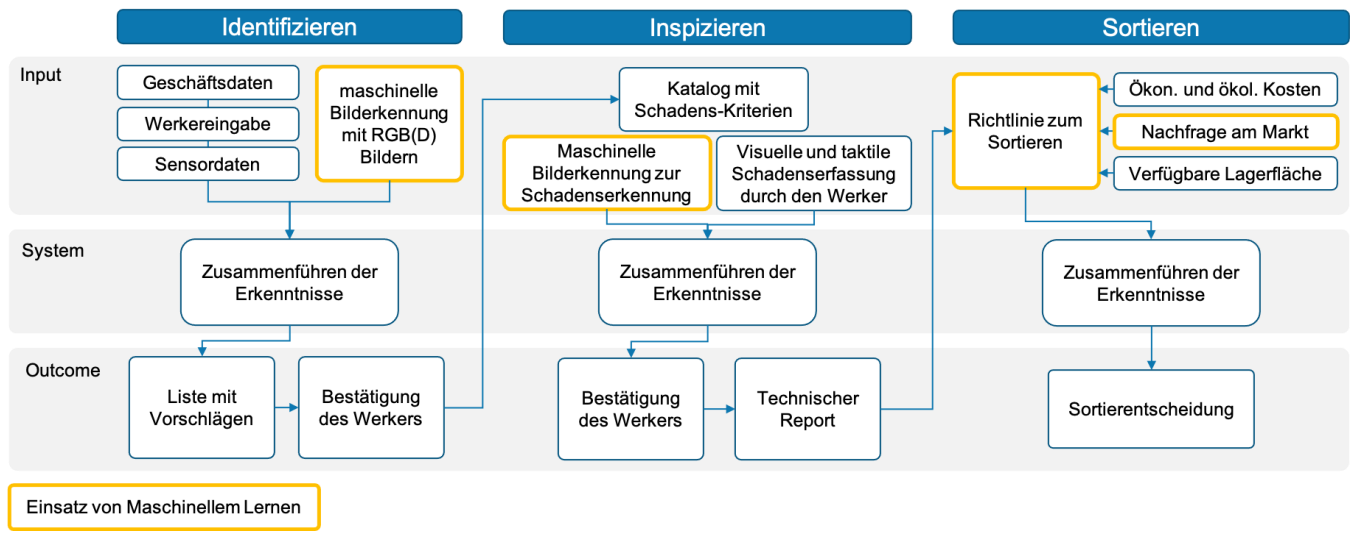
\includegraphics[width=\textwidth]{images/figure_eiba_process.png}
%	\caption[Integration des in EIBA entwickelten KI-gestützten Systems in den Prozess der Indentifikation, Inspektion und Sortierung von Altteilen.]{Integration des in EIBA entwickelten KI-gestützten Systems\\
%	in den Prozess der Indentifikation, Inspektion und Sortierung\\
%	von Altteilen \parencite{Wagner2022reziprok}.}
%	\label{fig:eiba-process}
%\end{figure}
\begin{figure}[b!]
	\centering
	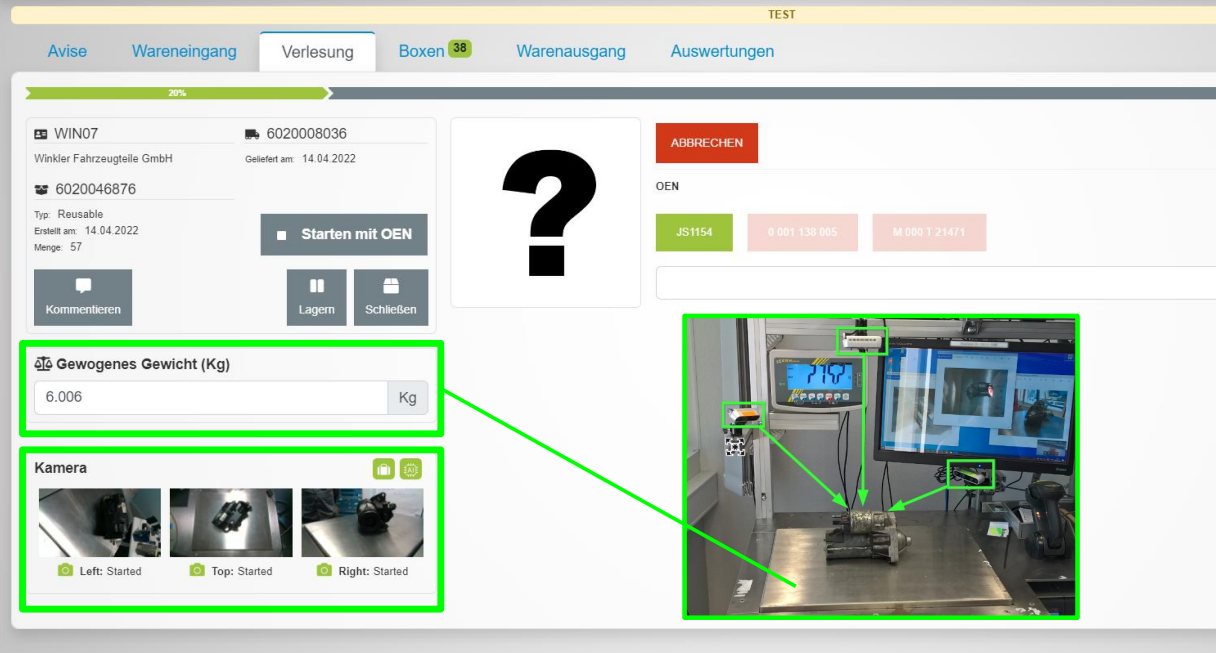
\includegraphics[width=\textwidth]{images/figure_eiba_interface.png}
	\caption[Die Mensch-Maschine-Schnittstelle des EIBA-Systems.]{Die Mensch-Maschine-Schnittstelle des EIBA-Systems \parencite{Wagner2022reziprok}.}
	\label{fig:eiba-interface}
\end{figure}

Viele der Altteile sind sehr ähnlich und erfordern Expertenwissen, um sie korrekt zu identifizieren und den Beschädigungsgrad zu bewerten, wobei die Beschriftungen und Barcodes oft nicht mehr lesbar sind. Hier setzt das KI-System an, um den Menschen zu unterstützen. Es werden dafür multimodale Sensordaten verwendet, unter anderem Tiefenkameras (RGB-D) und eine Waage zur Erfassung des Gewichts zum Einsatz. In \autoref{fig:eiba-interface} ist die Mensch-Maschine-Schnittstelle einer mobilen Teststation des Systems dargestellt.

% Ergebnisse vielversprechend, aber vorerst nur im Labor; Generalisierung verbessern
Das System konnte am Beispiel von gebrauchten Fahrzeugteilen bereits eine gute Accuracy erreichen. Die Beschaffung einer ausreichenden Menge an Beispielbildern\textemdash sowohl für das Training als auch für die Validierung\textemdash meist jedoch äußerst schwierig. Dadurch werden die Objektklassen nicht mit ausreichend Variation repräsentiert, was die Generalisierungsfähigkeit der Modelle beeinträchtigen könnte.

\subsection{Herausforderungen bei der Generierung synthetischer Daten} \label{subsec:challenges-synt-data}

Um die Datenvielfalt zu erhöhen, bietet sich die Generierung von synthetischen Daten an. Dabei steht vor allem die Darstellung unterschiedlicher Gebrauchszustände im Vordergrund, die in der Realität nur schwer zu beschaffen sind. In \autoref{sec:synt-data} wurden bereits verschiedene Methoden zur Bildgenerierung vorgestellt, die sich für diesen Zweck eignen. Dabei ergeben sich jedoch eine Reihe von Herausforderungen, die bereits in der Einleitung angesprochen wurden.

Der Anwendungsfall zeichnet sich durch folgende Eigenschaften aus, die die Generierung synthetischer Daten erschweren:

\begin{enumerate}
	\item Die Objekte weisen teilweise eine sehr hohe Komplexität auf, etwa bei Motoren oder Generatoren mit vielen Details. 
	\item Es gibt oft nur feine Unterschiede zwischen den Klassen, die es zu berücksichtigen gilt.
	\item Die Bilder haben nur wenig Variation, vor allem in den Hintergründen. Auch die Objekte selbst sind zwar aus verschiedenen Perspektiven aufgenommen, bieten aber pro Klasse nicht viel Variation.
\end{enumerate}

Dies führt bei der Verwendung herkömmlicher Methoden zur synthetischen Datengenerierung zu Problemen. Einerseits scheitern viele dieser Methoden bei der Generierung komplexer Konzepte \parencite{Lu2024syntheticdatareview}, was aufgrund der feinen Unterschiede zwischen den Klassen besonders problematisch ist. Auch die Verwendung von "Off-the-shelf"-Modellen zur T2I-Generierung sind deshalb oft nicht in der Lage spezifische Konzepte eines Anwendungsfalls akkurat wiederzugeben \parencite{Fan2023scalingsyntheticimages}. Wenn synthetische Daten mit mangelhafter Qualität auf naive Weise in das Training integriert werden, kann sich dann die Leistung der Modelle verschlechtern \parencite{VanBreugel2023syntheticdatarealerrors}.

Es ergeben sich also hohe Anforderungen. Einerseits muss die Genauigkeit der generierten Daten gewährleistet sein, um die Klassifikation der Modelle nicht zu beeinträchtigen. Andererseits muss genügend Variation ermöglicht werden, um die Generalisierungsfähigkeit der Modelle zu verbessern.

DA-Fusion soll deshalb in dieser Arbeit als Methode zur Generierung synthetischer Daten untersucht werden. Sie bietet womöglich eine Lösung für die genannten Probleme, indem die Bilder nicht von Grund auf neu generiert werden, sondern die Struktur der echten Daten beibehalten. Dadurch könnte die Genauigkeit der generierten Daten erhöht und gleichzeitig die Variation der Daten verbessert werden.

\subsection{Synthetische Daten als negativ-Beispiele im Contrastive Learning} \label{subsec:synt-ood-contrastive}

% Herausforderungen -> Forschungslücke ?
Neben der Generierung von synthetischen Daten stellt sich die Frage, wie diese effektiv in das Training von Modellen integriert werden können.

Mit Blick auf die Herausforderungen bei der Generierung synthetischer Daten, zusammen mit den Besonderheiten des Contrastive Learning, ergibt sich eine interessante Forschungslücke: Ist es möglich, auch aus \emph{mangelhaften} synthetischen Daten zu lernen, wenn sie ausschließlich als negativ-Beispiele im Contrastive Learning verwendet werden? Lässt sich so die Leistung eines Modells bei der Klassifikation von echten Daten verbessern und gleichzeitig die Robustheit gegenüber OOD-Daten erhöhen?

Bisherige Ansätze im Contrastive Learning, wie etwa \parencite{Khosla2021supcon}, haben sich weitgehend auf reale Daten als negative Beispiele verlassen. Die Idee, synthetische Daten gezielt als negativ-Beispiele zu nutzen, stellt einen neuen Ansatz dar. Dies könnte besonders dann interessant sein, wenn die generierten OOD-Daten visuell ähnlich zu den ID-Daten sind. Solche Near OOD-Daten könnten für die ID-Daten eine ähnliche Funktion wie Hard Negatives erfüllen und gleichzeitig die Fehlklassifikation von OOD-Daten reduzieren.

% SimCLR profitierte besonders von hard negatives; Synt. Daten dürfen also nicht zu entfernt sein
Die bisherigen Erfolge von Contrastive Learning, insbesondere von SimCLR, zeigen, dass das Modell von Hard Negatives besonders stark profitiert \parencite{Chen2020simclr}. Auch \parencite{Jiang2024supconhardnegatives} baut auf dieser Erkenntnis auf und führt eine Strategie zum Hard Negative Sampling im Supervised Contrastive Learning ein\textemdash jedoch ohne Verwendung von synthetischen Daten.

Es gilt also zu untersuchen, ob ein Modell durch den Einsatz von synthetischen negativ-Beispielen, die mittels Diffusionsmodellen oder ähnlichen Techniken generiert wurden, seine Fähigkeit zur Generalisierung verbessern kann. Insbesondere stellt sich die Frage, ob diese synthetischen Daten die Robustheit gegenüber echten OOD-Daten erhöhen können.

\subsection{Integration von DA-Fusion und Supervised Contrastive Learning} \label{subsec:da-fusion-supcon}

Im Rahmen dieser Arbeit wird ein Ansatz vorgestellt, bei dem synthetische Augmentationen, die mit DA-Fusion generiert wurden, gezielt in das Supervised Contrastive Learning eingebunden werden. Die Grundidee besteht darin, sowohl ID-Daten (In-Distribution) als auch Near OOD-Daten (Near Out-of-Distribution) durch eine kontrollierte Anpassung der Augmentationsstärke zu erzeugen. Die Near OOD-Daten werden dabei im Contrastive Learning als Hard Negatives verwendet, um die Repräsentationen des Modells zu verbessern.

% DA-Fusion; strength-Parameter
Wie bereits erwähnt, ist DA-Fusion für die Generierung von Augmentationen vielversprechend. Durch die Erhöhung des Parameters für die Augmentationsstärke können zunehmend variierende Beispiele generiert werden. Für die ID-Daten wird eine moderate Augmentationsstärke verwendet. Demgegenüber werden die Near OOD-Daten durch eine stärkere Augmentation erzeugt, wobei noch ausreichend Ähnlichkeit zu den ID-Daten bestehen bleibt, um als Hard Negative zu gelten.

% Supervised Contrastive Learning mit eigener Sampling-Strategie
Im Kontext des Supervised Contrastive Learning wird eine eigene Sampling-Strategie für Near OOD-Daten entwickelt. Diese Daten werden nicht wahllos als negativ-Beispiele verwendet, sondern gezielt aus den Augmentationen derselben Klasse des Ankerbeispiels ausgewählt. Dies stellt sicher, dass die negativen Beispiele in den gleichen semantischen Raum fallen, aber durch die Augmentationen genug variieren, um als OOD-Daten zu gelten. Die Idee ist, dass so feinere Unterschiede innerhalb und außerhalb der Klasse gelernt werden, wodurch die Generalisierungsfähigkeit gegenüber realen Daten verbessert wird.

Die Formulierung der Verlustfunktion aus dem Supervised Contrastive Learning in \autoref{eq:loss-supcon} wird entsprechend der Verwendung von Near OOD-Daten in \autoref{eq:loss-da-fusion-supcon} leicht angepasst.

\begin{equation}
	Loss = - \sum_{i=1}^{N} \log \left( \frac{1}{|\text{P}(i)|} \sum_{p \in \text{P}(i)} \frac{\exp(s_{i,p}/\tau)}{\sum_{j \in \text{J}(i)} \exp(s_{i,j}/\tau)} \right),
	\label{eq:loss-da-fusion-supcon}
\end{equation} % \frac{1}{N}

wobei $\text{J}(i)$ die negativ-Beispiele für das Ankerbeispiel $i$ sind (ID und OOD), welche gefiltert wurden, um von den OOD-Augmentationen nur solche zu verwenden, die aus der Klasse des Ankerbeispiels generiert wurden und somit als Near OOD gelten.